\section{Procesy i zarządzanie procesami}

\subsection{Wstęp}

Przykłady procesów w życiu codziennym: proces fizyczny, chemiczny,
technologiczny, proces sądowy, administracyjny. Proces to przebieg powiązanych
ze sobą zmian. Większość procesów zachodzi w~określonym środowisku (np.
w~urzędzie), podlega pewnym ograniczeniom (np.  procedurom prawnym) i~wymaga
pewnych zasobów (np.  pieniędzy podatników). Pewne zdarzenia w~procesie
mogą występować sekwencyjnie, inne mogą nakładać się na siebie w~czasie. Jeśli
jesteśmy w~stanie wyodrębnić unikalny ciąg występujących po sobie zdarzeń
i~stwierdzić, że są ze sobą jakoś powiązane, to taką sekwencję często określa
się mianem wątku. Proces, podobnie jak fabuła powieści, może obejmować wiele
wątków biegnących równocześnie.

W~informatyce proces jest dynamicznym obiektem utworzonym przez system
operacyjny w~celu wykonania pewnego programu. Procesowi przydzielane są zasoby
takie jak czas procesora, obszar pamięci operacyjnej, pliki, urządzenia
peryferyjne. W~pamięci komputera zwykle znajduje się wiele procesów, które są
na różnych etapach wykonania i~współzawodniczą o~zasoby. W~obrębie jednego
procesu występuje jeden lub więcej wątków (w uproszczeniu wątek obrazuje ciąg
wykonywanych po sobie instrukcji procesora), wątki mogą być wykonywane
równolegle (tj. wątek A biegnie równolegle z~wątkiem B).

Często proces jest utożsamiany z~programem uruchomionym w~systemie operacyjnym.
Rzeczywiste aplikacje mogą się jednak składać z~wielu procesów, które
komunikują się ze sobą za pomocą mechanizmów komunikacji międzyprocesowej
(inter-process communication, IPC). Zagadnieniom komunikacji IPC poświęcono
odrębne rozdziały tej instrukcji.

Obiekt-proces (tak jak większość obiektów w~informatyce) posiada pewne atrybuty,
oraz podlega regułom określającym jego czas życia. W~niniejszym laboratorium
omówimy następujące zagadnienia:
\begin{myitemize}
  \item wyświetlanie i~modyfikowanie atrybutów procesów (atrybuty),
  \item tworzenie i usuwanie procesów (czas życia).
\end{myitemize}

\subsection{Wyświetlanie i modyfikowanie atrybutów procesów}

Atrybuty to informacje przechowywane przez obiekt-proces na rzecz systemu
operacyjnego. Pozwalają systemowi i~użytkownikowi identyfikować procesy oraz
np. określać jakie zasoby są aktualnie przydzielone poszczególnym procesom.

Każdy proces w systemie QNX ma przypisany unikalny identyfikator PID (process
ID), który jest liczbą całkowitą. Każdy proces (oprócz procesu ,,głównego''
\texttt{procnto}) ma również swój proces macierzysty. Identyfikator PPID
(parent process ID) jest identyfikatorem PID procesu macierzystego. Proces
\texttt{procnto} ma identyfikator PID=1 i~nie ma identyfikatora PPID. Wybrane
atrybuty i~funkcje systemowe umożliwiające dostęp do nich przedstawiono
w~tabeli \ref{tab:HE6LE}.

%%%%%%%%%%%%%%%%%%%%%%%%%%%%%%%%%%%%%%%%%%%%%%%%%%%%%%%%%%%%%%%%%%%%%%%%%%%%%
\begin{table}[h!]
  \centering
  \caption{Niektóre atrybuty procesów oraz funkcje biblioteki systemowej
           umożliwiające dostęp do nich}
  \label{tab:HE6LE}
  \begin{tabular}{|c|c|c|}
    \hline
    \textbf{Atrybuty procesu} & \textbf{Wyświetlanie} & \textbf{Modyfikacja} \\ \hline
    Identyfikator PID                   & \texttt{getpid()}           & -- \\ \hline
    Identyfikator PPID                  & \texttt{getppid()}          & -- \\ \hline
    Priorytet i~strategia szeregowania  & \texttt{sched\_getparam()}  & \texttt{sched\_setparam()} \\ \hline
  \end{tabular}
\end{table}
%%%%%%%%%%%%%%%%%%%%%%%%%%%%%%%%%%%%%%%%%%%%%%%%%%%%%%%%%%%%%%%%%%%%%%%%%%%%%

Na ogół mamy do czynienia z sytuacją, kiedy procesów gotowych do wykonania jest
więcej niż umożliwiają to dostępne w~danej chwili zasoby. Procedura szeregująca
(scheduler) rozstrzyga, któremu z procesów (wątków) zostanie w~danej chwili
przydzielony czas procesora. Jednym z~istotnych parametrów rzutujących na
kolejność przydzielania czasu procesora jest priorytet -- każdy z procesów (i
wątków -- patrz następne laboratoria) ma przyporządkowany priorytet (process
priority).  Jest on miarą pilności wykonania danego procesu względem innych.
W systemie QNX Neutrino 6 priorytet jest liczbą z zakresu od 0 (najniższy) do
255 (najwyższy). System nakłada ograniczenia na dopuszczalne zakresy
priorytetów dla programów uruchamianych przez poszczególnych użytkowników
(tabela \ref{tab:2N6W7}):

%%%%%%%%%%%%%%%%%%%%%%%%%%%%%%%%%%%%%%%%%%%%%%%%%%%%%%%%%%%%%%%%%%%%%%%%%%%%%
\begin{table}[h!]
  \centering
  \caption{Priorytety w~QNX Neutrino 6}
  \label{tab:2N6W7}
  \begin{tabular}{|c|c|c|}
    \hline
    \textbf{Priorytet} & \textbf{Użytkownik} \\ \hline
    0 & Proces jałowy \\ \hline
    1 -- 63 & Wątki zwykłego użytkownika \\ \hline
    1 -- 255 & Wątki użytkownika \texttt{root} \\ \hline
  \end{tabular}
\end{table}
%%%%%%%%%%%%%%%%%%%%%%%%%%%%%%%%%%%%%%%%%%%%%%%%%%%%%%%%%%%%%%%%%%%%%%%%%%%%%

W systemie QNX są dostępne trzy strategie szeregowania:
\begin{myitemize}
  \item szeregowanie FIFO (FIFO scheduling),
  \item szeregowanie karuzelowe (round robin scheduling),
  \item szeregowanie sporadyczne (sporadic scheduling).
\end{myitemize}
Są one omówione szczegółowo w dokumentacji QNX~\cite{qnx}. W tabeli
\ref{tab:A9C2X} przedstawiono ich symbole, wykorzystywane w~wywołaniach
systemowych.


%%%%%%%%%%%%%%%%%%%%%%%%%%%%%%%%%%%%%%%%%%%%%%%%%%%%%%%%%%%%%%%%%%%%%%%%%%%%%
\begin{table}[h!]
  \centering
  \caption{Strategie szeregowania w~QNX Neutrino 6}
  \label{tab:A9C2X}
  \begin{tabular}{|c|c|c|}
    \hline
    \textbf{Symbol}           & \textbf{Opis} \\ \hline
    \texttt{SCHED\_FIFO}      & Szeregowanie FIFO \\ \hline
    \texttt{SCHED\_RR}        & Szeregowanie karuzelowe \\ \hline
    \texttt{SCHED\_SPORADIC}  & Szeregowanie sporadyczne \\ \hline
  \end{tabular}
\end{table}
%%%%%%%%%%%%%%%%%%%%%%%%%%%%%%%%%%%%%%%%%%%%%%%%%%%%%%%%%%%%%%%%%%%%%%%%%%%%%

%%%%%%%%%%%%%%%%%%%%%%%%%%%%%%%%%%%%%%%%%%%%%%%%%%%%%%%%%%%%%%%%%%%%%%%%%%%%%
\begin{example}{[Lista procesów]}
  \label{ex:TYRDA}
  W terminalu wykonać polecenie \texttt{ps -l}. Sprawdzić w {\color{red}dokumentacji},
  co oznaczają poszczególne kolumny wyświetlonego raportu.
\end{example}
%%%%%%%%%%%%%%%%%%%%%%%%%%%%%%%%%%%%%%%%%%%%%%%%%%%%%%%%%%%%%%%%%%%%%%%%%%%%%

%%%%%%%%%%%%%%%%%%%%%%%%%%%%%%%%%%%%%%%%%%%%%%%%%%%%%%%%%%%%%%%%%%%%%%%%%%%%%
\begin{example}{[Wyświetlanie i modyfikacja wybranych atrybutów procesu]}
  \label{ex:TEPBG}
  \lstinputlisting[style=MyCStyle,label=src:4JKQ7]{src/lab4/attributes1.c}
\end{example}
%%%%%%%%%%%%%%%%%%%%%%%%%%%%%%%%%%%%%%%%%%%%%%%%%%%%%%%%%%%%%%%%%%%%%%%%%%%%%


\subsection{Tworzenie procesów}

W systemie QNX Neutrino, modułem odpowiedzialnym za dynamiczne tworzenie,
usuwanie oraz zarządzanie procesami jest zawarty w mikrojądrze (procnto)
manager procesów. W systemie QNX istnieją różne metody tworzenia procesów.
Część z nich pochodzi wprost od systemów UNIX-owych, opartych o standard POSIX,
inne funkcje do tworzenia procesów są charakterystyczne tylko dla systemu QNX.
Podstawowe funkcje do tworzenia procesów przedstawiono w tabeli
\ref{tab:IMJR3}. W ramach laboratorium omówimy cztery funkcje, służące
tworzeniu procesów, tj. \texttt{system()}, \texttt{fork()}, \texttt{exec()},
\texttt{spawn()}.

%%%%%%%%%%%%%%%%%%%%%%%%%%%%%%%%%%%%%%%%%%%%%%%%%%%%%%%%%%%%%%%%%%%%%%%%%%%%%
\begin{table}[h!]
  \centering
  \caption{Metody tworzenia procesów w systemie QNX}
  \label{tab:IMJR3}
  \begin{tabular}{|l|p{0.75\textwidth}|}
    \hline
    \textbf{Funkcja}    & \textbf{Opis}  \\ \hline
    \texttt{system()}   & Wywołanie programów, poleceń systemowych, bądź skryptów \\ \hline
    \texttt{fork()}     & Utworzenie kopii procesu bieżącego \\ \hline
    \texttt{exec()}     & Zastąpienie bieżącego procesu nowym procesem -- rodzina funkcji \\ \hline
    \texttt{spawn()}    & Utworzenie procesu potomnego -- rodzina funkcji \\ \hline
    \texttt{vfork()}    & Utworzenie procesu potomnego i zablokowanie procesu macierzystego \\ \hline
    \texttt{forkpty()}  & Utworzenie procesu potomnego w oknie pseudoterminala \\ \hline
    \texttt{popen()}    & Uruchomienie programu jako procesu potomnego z
                          jednoczesnym utworzeniem łącza pomiędzy procesem
                          bieżącym, a potomnym \\ \hline
  \end{tabular}
\end{table}
%%%%%%%%%%%%%%%%%%%%%%%%%%%%%%%%%%%%%%%%%%%%%%%%%%%%%%%%%%%%%%%%%%%%%%%%%%%%%

Jednym z~najprostszych sposobów uruchomienia innego procesu z~poziomu programu
w~języku C jest użycie funkcji \texttt{system()} (przykład \ref{ex:V86MA}).
Poleceniem tym można uruchomić program w~sposób podobny, jak to się czyni
wprost z~powłoki. Funkcja zwraca status zakończenia uruchomionego programu.

%%%%%%%%%%%%%%%%%%%%%%%%%%%%%%%%%%%%%%%%%%%%%%%%%%%%%%%%%%%%%%%%%%%%%%%%%%%%%
\begin{example}{[Wywołanie programu za pomocą polecenia system()]}
  \label{ex:V86MA}
  \lstinputlisting[style=MyCStyle,label=src:P1A10]{src/lab4/system1.c}
\end{example}
%%%%%%%%%%%%%%%%%%%%%%%%%%%%%%%%%%%%%%%%%%%%%%%%%%%%%%%%%%%%%%%%%%%%%%%%%%%%%

Funkcja \texttt{fork()} tworzy kopię procesu i~uruchamia ją jako proces
potomny. Utworzony proces potomny wykonuje się współbieżnie z procesem
tworzącym, posiada własny nr PID, a jego PPID wskazuje na proces tworzący.
Funkcja \texttt{fork()} tworzy deskryptor nowego procesu oraz kopię segmentu
kodu, danych i stosu. Modyfikacje zmiennych w procesie macierzystym nie są
widoczne w procesie potomnym i odwrotnie. Jeżeli operacja utworzenia procesu
potomnego zakończy się powodzeniem, to funkcja w procesie macierzystym zwraca
identyfikator (PID) procesu potomnego (wartość większa od 1), a w procesie
potomnym wartość 0. Jeżeli próba utworzenia procesu się nie powiedzie, to
funkcja \texttt{fork()} zwraca w procesie macierzystym wartość -1. Działanie
funkcji przedstawiono na rysunku, a jej użycie w przykładzie~\ref{ex:HP9M8}.

%%%%%%%%%%%%%%%%%%%%%%%%%%%%%%%%%%%%%%%%%%%%%%%%%%%%%%%%%%%%%%%%%%%%%%%%%%%%%
\begin{figure}
  \centering
  \begin{tikzpicture}
    \node[TBox6emCentered] (parent)   at (0.00,3.50)  {Proces macierzysty};
    \node                  (fork)     at (0.00,1.75)  {\texttt{fork()}};
    \node                  (x)        at (4.50,1.75)  {};
    \node[TBox6emCentered] (parent2)  at (0.00,0.00)  {Proces macierzysty};
    \node[TBox6emCentered] (child)    at (4.50,0.00)  {Proces potomny};

    \draw[->] (parent.south)  to                                                (fork.north);
    \draw[->] (fork.south)    to node[anchor=center,left]{Zwraca PID potomka}   (parent2.north);
    \draw[->] (fork.east)     to                                                (x.center)
                              to node[anchor=center, right]{Zwraca zero}        (child.north);
  \end{tikzpicture}
  \caption{Idea działania funkcji \texttt{fork()}}
  \label{fig:S278F}
\end{figure}
%%%%%%%%%%%%%%%%%%%%%%%%%%%%%%%%%%%%%%%%%%%%%%%%%%%%%%%%%%%%%%%%%%%%%%%%%%%%%

%%%%%%%%%%%%%%%%%%%%%%%%%%%%%%%%%%%%%%%%%%%%%%%%%%%%%%%%%%%%%%%%%%%%%%%%%%%%%
\begin{example}{[Wywołanie funkcji fork()]}
  \label{ex:HP9M8}
  \lstinputlisting[style=MyCStyle,label=src:P1A10]{src/lab4/fork1.c}

  Sprawdzić działanie programu, gdy zmienna CHILD = 8, a zmienna PARENT = 4.
\end{example}
%%%%%%%%%%%%%%%%%%%%%%%%%%%%%%%%%%%%%%%%%%%%%%%%%%%%%%%%%%%%%%%%%%%%%%%%%%%%%

\subsection{Obsługa zakończenia procesów}

Poprawne zakończenie procesów jest zagadnieniem, na które należy zwrócić
szczególną uwagę przy rozwoju wiarygodnego oprogramowania w systemie QNX.
Powodem tego jest fakt, że procesy na ogół współdziałają ze sobą, mogą być np.
procesami macierzystymi, bądź oczekiwać na określone zdarzenia, wygenerowane
przez inne procesy. W związku z tym, przed zakończeniem procesu należy zwolnić
zajęte przez ten proces zasoby, zakończyć z innymi procesami scenariusze
komunikacyjne i synchronizacyjne oraz zaczekać na zakończenie procesów
potomnych.

Zakończenie procesu następuje w następujących przypadkach:
\begin{myitemize}
  \item poprzez wywołanie funkcji exit(),
  \item funkcja main() wywołuje instrukcję return lub zakończyło się działanie
        ostatniej instrukcji kodu,
  \item proces zostanie zakończony przez system operacyjny lub inny proces.
\end{myitemize}

Normalne zakończenie procesu może być zainicjowane przez programistę, poprzez
wywołanie funkcji \texttt{exit()}

%%%%%%%%%%%%%%%%%%%%%%%%%%%%%%%%%%%%%%%%%%%%%%%%%%%%%%%%%%%%%%%%%%%%%%%%%%%%%
\begin{lstlisting}[style=MyCStyle]
 #include <stdlib.h>
 void exit( int status );
\end{lstlisting}
%%%%%%%%%%%%%%%%%%%%%%%%%%%%%%%%%%%%%%%%%%%%%%%%%%%%%%%%%%%%%%%%%%%%%%%%%%%%%

Funkcja ta powoduje zakończenie procesu bieżącego oraz zwrócenie statusu
zakończonego procesu.  Status jest dostępny dla procesu macierzystego. Na ogół
wartość statusu jest ustawiana na \texttt{EXIT\_SUCCESS}, gdy proces zakończył
się poprawnie, bądź na wartość \texttt{EXIT\_FAILURE}, bądź innych kod, gdy
wystąpił błąd.

W przypadku, gdy proces macierzysty uruchamia procesy potomne, należy unikać
sytuacji, gdy proces macierzysty kończy się wcześniej, niż jego procesy potomne
(osierocenie procesów). Proces macierzysty powinien zaczekać na zakończenie
swoich procesów potomnych. Do synchronizacji zakończenia procesów używa się
funkcji:


%%%%%%%%%%%%%%%%%%%%%%%%%%%%%%%%%%%%%%%%%%%%%%%%%%%%%%%%%%%%%%%%%%%%%%%%%%%%%
\begin{lstlisting}[style=MyCStyle]
  #include <sys/types.h>
  #include <sys/wait.h>
  pid_t wait( int * status );
\end{lstlisting}
%%%%%%%%%%%%%%%%%%%%%%%%%%%%%%%%%%%%%%%%%%%%%%%%%%%%%%%%%%%%%%%%%%%%%%%%%%%%%

Zmienna \texttt{status} jest statusem zakończenia procesu potomnego. Funkcja
zwraca PID zakończonego procesu, bądź -1, w przypadku gdy brak procesów
potomnych. \texttt{wait()} blokuje proces wywołujący, do momentu, gdy któryś z procesów
potomnych zakończył się poprawnie (np. wywołał funkcję \texttt{exit()}), bądź
wystąpił błąd.

%%%%%%%%%%%%%%%%%%%%%%%%%%%%%%%%%%%%%%%%%%%%%%%%%%%%%%%%%%%%%%%%%%%%%%%%%%%%%
\begin{figure}
  \centering
  \begin{tikzpicture}
    \node[TBox6emCentered]  (parent)  at (0.00, 3.50) {Proces macierzysty};
    \node                   (fork)    at (0.00, 2.00) {\texttt{fork()}};
    \node                   (wait)    at (0.00, 0.75) {\texttt{wait()}};
    \node[TBox6emCentered]  (child)   at (4.50, 2.00) {Proces potomny};
    \node[circle,draw=black](o)       at (0.00,-0.25) {};
    \node                   (exit)    at (4.50,-0.25) {\texttt{exit()}};
    \node                   (end1)    at (0.00,-1.00) {};
    \node[circle,fill=black](end2)    at (4.50,-1.00) {};
    \node[right of = end2]  (end2t)   {Koniec};

    \draw[->] (parent.south)  to (fork.north);
    \draw[->] (fork.east)     to (child.west);
    \draw[->] (fork.south)    to (wait.north);
    \draw[->] (wait.south)    to node[anchor=center,left]{Oczekiwanie} (o.north);
    \draw[->] (child.south)   to (exit.north);
    \draw[->,dotted] (exit.west)     to (o.east);
    \draw[->] (o.south)       to node[anchor=center,left]{Dalszy bieg} (end1.south);
    \draw[->] (exit.south)    to (end2);
  \end{tikzpicture}
  \caption{Schemat poprawnego zakończenia procesu}
  \label{fig:Z6B8G}
\end{figure}
%%%%%%%%%%%%%%%%%%%%%%%%%%%%%%%%%%%%%%%%%%%%%%%%%%%%%%%%%%%%%%%%%%%%%%%%%%%%%

Ilustrację omawianych zagadnień stanowi niniejszy przykład.

%%%%%%%%%%%%%%%%%%%%%%%%%%%%%%%%%%%%%%%%%%%%%%%%%%%%%%%%%%%%%%%%%%%%%%%%%%%%%
\begin{example}{[Wywołanie funkcji fork() wraz z obsługą zakończenia procesów]}
  \label{ex:11SSB}
  \lstinputlisting[style=MyCStyle,label=src:92W6D]{src/lab4/process1.c}
\end{example}
%%%%%%%%%%%%%%%%%%%%%%%%%%%%%%%%%%%%%%%%%%%%%%%%%%%%%%%%%%%%%%%%%%%%%%%%%%%%%


Zastosowanie funkcji \texttt{wait()} zapewnia, że proces macierzysty nie zakończy się
przed procesem potomnym. W przypadku, gdy proces potomny zakończy się przed
wywołaniem przez macierzysty funkcji \texttt{wait()}, proces potomny zwalnia
wszystkie zasoby, z wyjątkiem deskryptora procesu, czyli miejsca w pamięci
operacyjnej, gdzie przechowywane są wszystkie informacje potrzebne do
zarządzania procesem. Status zakończenia procesu potomnego jest przekazywany do
procesu macierzystego w deskryptorze procesu potomnego. Taki stan procesu
potomnego nazywa się stanem ,,zombie''.

Inną funkcją, pozwalającą na oczekiwanie na zakończenie konkretnego procesu
potomnego jest funkcja \texttt{waitpid()}.

%%%%%%%%%%%%%%%%%%%%%%%%%%%%%%%%%%%%%%%%%%%%%%%%%%%%%%%%%%%%%%%%%%%%%%%%%%%%%
\begin{lstlisting}[style=MyCStyle]
#include <sys/types.h>
#include <sys/wait.h>

pid_t waitpid( pid_t pid, int *status, int options );
\end{lstlisting}
%%%%%%%%%%%%%%%%%%%%%%%%%%%%%%%%%%%%%%%%%%%%%%%%%%%%%%%%%%%%%%%%%%%%%%%%%%%%%

Funkcja zwraca PID zakończonego procesu, bądź -1, w przypadku, gdy brak jest
procesów potomnych. Funkcja zwraca również status zakończonego procesu poprzez
argument \texttt{status}. Jedną z użytecznych opcji funkcji jest flaga
\texttt{WNOHANG}, która powoduje, że proces macierzysty, w przypadku braku
potomnych, natychmiast wraca z funkcji i kontynuuje swoje działanie i w tym
przypadku możemy użyć takiej kombinacji do cyklicznego sprawdzania, czy proces
potomny się zakończył.


\subsection{Zastąpienie procesu bieżącego innymi procesami}

Funkcje z rodziny exec() zastępują bieżący proces, nowym procesem, na podstawie
pliku wykonywalnego, którego nazwa jest parametrem funkcji. W odróżnieniu od
funkcji \texttt{fork()},  w przypadku użytkowania funkcji z rodziny
\texttt{exec()}, kody procesów macierzystych i potomnych mogą być umieszczone w
oddzielnych plikach źródłowych. Taka konfiguracja zapewnia łatwiejsze
uruchamianie i testowanie programów. W systemie QNX zdefiniowano następującą
rodzinę funkcji: \texttt{execl()}, \texttt{execle()}, \texttt{execlp()},
\texttt{execlpe()}, \texttt{execv()}, \texttt{execve()}, \texttt{execvp()},
\texttt{execvpe()}. Działanie tych funkcji jest podobne, natomiast różnią się
listą parametrów formalnych. W trakcie laboratorium będziemy używać
najprostszych funkcji \texttt{execl()} oraz \texttt{execv()}, których sygnatury
wyglądają następująco:

%%%%%%%%%%%%%%%%%%%%%%%%%%%%%%%%%%%%%%%%%%%%%%%%%%%%%%%%%%%%%%%%%%%%%%%%%%%%%
\begin{lstlisting}[style=MyCStyle]
#include <process.h>

int execl(  const char * path,
            const char * arg0,
            const char * arg1,
            ...
            const char * argn,
            NULL );
int execv( const char * path,
           char * const argv[] );
\end{lstlisting}
%%%%%%%%%%%%%%%%%%%%%%%%%%%%%%%%%%%%%%%%%%%%%%%%%%%%%%%%%%%%%%%%%%%%%%%%%%%%%

gdzie \texttt{path} jest ścieżką do pliku wykonywalnego, a argumenty
\texttt{arg[0]} do \texttt{arg[n]} -- nazwą i argumentami programu. Na ostatnim
miejscu podaje się wartość \texttt{NULL}, na oznaczenie zakończenia listy
parametrów wywoływanego programu.

Funkcja \texttt{execv()} pobiera tylko dwa argumenty i daje możliwość
elastycznego budowania listy parametrów. Drugi z argumentów jest tablicą
napisów, która musi być zakończona pustym wskaźnikiem \texttt{((char *)0)}.
Wartość pola \texttt{argv[0]} musi wskazywać na nazwę procesu, który chcemy
uruchomić.

%%%%%%%%%%%%%%%%%%%%%%%%%%%%%%%%%%%%%%%%%%%%%%%%%%%%%%%%%%%%%%%%%%%%%%%%%%%%%
\begin{example}{[Wywołanie funkcji execl()]}
  \label{ex:WHF3V}
  \lstinputlisting[style=MyCStyle,label=src:5Y0UB]{src/lab4/execv1.c}
\end{example}
%%%%%%%%%%%%%%%%%%%%%%%%%%%%%%%%%%%%%%%%%%%%%%%%%%%%%%%%%%%%%%%%%%%%%%%%%%%%%

\subsection{Tworzenie procesów funkcją spawn()}

Posługiwanie się funkcjami \texttt{fork()} i \texttt{exec()} do tworzenia
procesów współbieżnych bywa niewygodne. System operacyjny QNX udostępnia
rodzinę \texttt{spawn()}, która służy do tworzenia procesów potomnych na
podstawie pliku wykonywalnego, którego nazwa jest jednym z argumentów funkcji.
Do tej grupy zaliczamy następujące funkcje: \texttt{spawn()},
\texttt{spawnl()}, \texttt{spawnv()}, \texttt{spawnle()}, \texttt{spawnlp()},
\texttt{spawnlpe()}, \texttt{spawnve()}, \texttt{spawnvp()},
\texttt{spawnvpe()}. Ponownie omówimy tylko dwie wybrane funkcje
\texttt{spawnl()} i~\texttt{spawnv()}, których deklaracje wyglądają
następująco:

%%%%%%%%%%%%%%%%%%%%%%%%%%%%%%%%%%%%%%%%%%%%%%%%%%%%%%%%%%%%%%%%%%%%%%%%%%%%%
\begin{lstlisting}[style=MyCStyle]
#include <process.h>

int spawnl( int mode,
            const char * path,
            const char * arg0,
            const char * arg1,
            ...
            const char * argn,
            NULL );
int spawnv( int mode,
            const char * path,
            char * const argv[] );
\end{lstlisting}
%%%%%%%%%%%%%%%%%%%%%%%%%%%%%%%%%%%%%%%%%%%%%%%%%%%%%%%%%%%%%%%%%%%%%%%%%%%%%
gdzie path jest ścieżką do pliku wykonywalnego, argumenty \texttt{arg[0]} do
\texttt{arg[n]} stanowią nazwę i argumenty programu. Ostatnim parametrem
funkcji jest string \texttt{NULL}, który służy do zakończenia listy parametrów
wywoływanego programu. Parametr mode jest trybem wykonania procesu. Tryb ten
mówi o sposobie wywołania procesu potomnego i metodzie zachowania procesu
macierzystego, gdy proces potomny zostanie zainicjowany.

Funkcja \texttt{spawnv()} pobiera trzy argumenty i daje możliwość elastycznego
budowania listy parametrów. Trzeci argument jest tablicą napisów, która musi być
zakończona pustym wskaźnikiem \texttt{((char *)0)}. Wartość pola
\texttt{argv[0]} musi wskazywać na nazwę procesu, który chcemy uruchomić.

%%%%%%%%%%%%%%%%%%%%%%%%%%%%%%%%%%%%%%%%%%%%%%%%%%%%%%%%%%%%%%%%%%%%%%%%%%%%%
\begin{table}
  \caption{Tryby wywołania funkcji \texttt{spawn()}}
  \label{tab:V0CUU}
  \begin{tabular}{|l|p{0.75\textwidth}|}
    \hline
    \textbf{Tryb}       & \textbf{Opis}
    \\ \hline
    \texttt{P\_WAIT}    & Proces macierzysty czeka na zakończenie procesu
                          potomnego i później jest kontynuowany.
    \\ \hline
    \texttt{P\_NOWAIT}  & Proces macierzysty i potomny są wykonywane
                          współbieżnie. Można używać funkcji \texttt{wait()}.
    \\ \hline
    \texttt{P\_NOWAITO} & Proces macierzysty i potomny są wykonywane
                          współbieżnie. Nie wolno używać funkcji wait() do
                          uzyskania kodu wyjścia. Relacja pokrewieństwa między
                          nimi zostaje przerwana.
    \\ \hline
    \texttt{P\_OVERLAY} & Proces macierzysty jest zastępowany przez proces
                          potomny. Wywołanie w tym trybie jest równoważne
                          wywołaniu funkcji execl().
    \\ \hline
  \end{tabular}
\end{table}
%%%%%%%%%%%%%%%%%%%%%%%%%%%%%%%%%%%%%%%%%%%%%%%%%%%%%%%%%%%%%%%%%%%%%%%%%%%%%

Ilustrację wywołania funkcji stanowi przykład:

%%%%%%%%%%%%%%%%%%%%%%%%%%%%%%%%%%%%%%%%%%%%%%%%%%%%%%%%%%%%%%%%%%%%%%%%%%%%%
\begin{example}{[Wywołanie funkcji spawnl()]}
  \label{ex:VSCD0}
  Utworzyć  dwa programy o nazwie macierzysty i potomny, następnie wywołać
  program macierzysty.
  \lstinputlisting[style=MyCStyle,label=src:4HNG2]{src/lab4/parent1.c}
  \lstinputlisting[style=MyCStyle,label=src:YZY1R]{src/lab4/child1.c}
\end{example}
%%%%%%%%%%%%%%%%%%%%%%%%%%%%%%%%%%%%%%%%%%%%%%%%%%%%%%%%%%%%%%%%%%%%%%%%%%%%%


\subsection{Ćwiczenia}

\begin{myenumerate}
  \item Napisać program, który tworzy dwa procesy. Każdy z procesów powinien
        utworzyć proces potomny. Wyświetlić identyfikatory procesów rodziców
        i~potomków.
  \item Napisać program, który tworzy proces macierzysty P1 i  potomny P2.
        Proces P2 uruchamia inny proces P3 za pomocą funkcji \texttt{execv()}.
        Parametry wywołania procesu P3 są przekazywane z wiersza poleceń.
  \item Utworzyć proces macierzysty mac, który stworzy za pomocą funkcji
        \texttt{fork()} 5 procesów potomnych oraz zaczekać na ich zakończenie.
        Niech każdy z procesów wyświetla co jedną sekundę swój numer PID, numer
        identyfikacyjny (w zależności od kolejności utworzenia) oraz czas
        działania. Czas działania poszczególnych procesów podawać jako
        argumenty do programu głównego (np.  mac 20 5 3 8 9). Na zakończenie
        procesu potomnego o nr i wywołać funkcję \texttt{exit(i)}. Proces
        macierzysty powinien czekać na zakończenie potomnych i wyświetlić
        informację, który z procesów potomnych się zakończył.
        %%%%%%%%%%%%%%%%%%%%%%%%%%%%%%%%%%%%%%%%%%%%%%%%%%%%%%%%%%%%%%%%%%%%%
        \begin{figure}[!h]
          \centering
          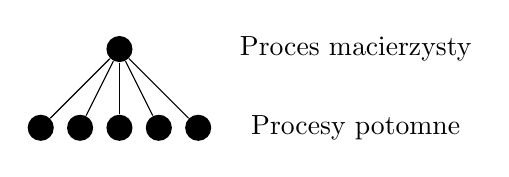
\begin{tikzpicture}
            \node[circle,fill=black] (o)  at ( 0.00, 0.00) {};
            \node[circle,fill=black] (c1) at (-1.00,-1.00) {};
            \node[circle,fill=black] (c2) at (-0.50,-1.00) {};
            \node[circle,fill=black] (c3) at (-0.00,-1.00) {};
            \node[circle,fill=black] (c4) at ( 0.50,-1.00) {};
            \node[circle,fill=black] (c5) at ( 1.00,-1.00) {};
            \node[] at (3.00,0.00) {Proces macierzysty};
            \node[] at (3.00,-1.00) {Procesy potomne};

            \draw[-]     (o) to (c1);
            \draw[-]     (o) to (c2);
            \draw[-]     (o) to (c3);
            \draw[-]     (o) to (c4);
            \draw[-]     (o) to (c5);
          \end{tikzpicture}
          \caption{Struktura 1-poziomowa}
          \label{fig:YT6VA}
        \end{figure}
        %%%%%%%%%%%%%%%%%%%%%%%%%%%%%%%%%%%%%%%%%%%%%%%%%%%%%%%%%%%%%%%%%%%%%

  \item Zadanie jest analogiczne do poprzedniego, z tym, że struktura procesów
        ma wyglądać jak drzewo przedstawione na rysunku \ref{fig:XDQ8Q}.
        %%%%%%%%%%%%%%%%%%%%%%%%%%%%%%%%%%%%%%%%%%%%%%%%%%%%%%%%%%%%%%%%%%%%%
        \begin{figure}[!h]
          \centering
          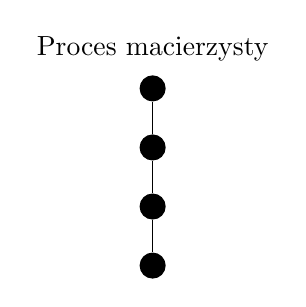
\begin{tikzpicture}
            \node[circle,fill=black] (c1) at ( 0.00, 2.25) {};
            \node[circle,fill=black] (c2) at ( 0.00, 1.50) {};
            \node[circle,fill=black] (c3) at ( 0.00, 0.75) {};
            \node[circle,fill=black] (c4) at ( 0.00, 0.00) {};
            \node[] at (0.00,2.75) {Proces macierzysty};

            \draw[-]     (c1) to (c2) to (c3) to (c4);
          \end{tikzpicture}
          \caption{Struktura 3-poziomowa}
          \label{fig:XDQ8Q}
        \end{figure}
        %%%%%%%%%%%%%%%%%%%%%%%%%%%%%%%%%%%%%%%%%%%%%%%%%%%%%%%%%%%%%%%%%%%%%
        Każdy z procesów, oprócz ostatniego tworzy jeden proces potomny.
\end{myenumerate}


\cleardoublepage

%% \label{??:7HOCC}
%% \label{??:3UDS1}
%% \label{??:BYA03}
%% \label{??:LDB7J}
%% \label{??:HXCTX}
%% \label{??:V35FU}
%% \label{??:V285P}
%% \label{??:0DR40}
%% \label{??:TFLMK}
%% \label{??:OD9EZ}
%% \label{??:87ILN}
%% \label{??:HY94T}
%% \label{??:GIWGJ}
%% \label{??:S0ENF}
%% \label{??:5O33M}
%% \label{??:9LCEW}
%% \label{??:FMIVT}
%% \label{??:8O5ZW}
%% \label{??:5GR5X}
%% \label{??:3KG12}
%% \label{??:O26C4}
%% \label{??:QXXWZ}
%% \label{??:FKPAJ}
%% \label{??:IUWYS}
%% \label{??:AKF4R}
%% \label{??:T7RU4}
%% \label{??:1QZGH}
%% \label{??:Z5EXB}
